\documentclass[a4paper,12pt]{article}
\usepackage[utf8]{inputenc}
\usepackage[T1]{fontenc}
\usepackage[british]{babel}
\usepackage{hyperref}
\usepackage[margin=1in]{geometry}
\usepackage{listings}
\usepackage{xspace}
\usepackage{graphicx}
\usepackage{indentfirst}

\title{Gomat specification}
\author{Gauthier Jolly \and K\'{e}vin Car\'{e}nou \and Matei Oltean}

\newcommand{\Gossiper}{\texttt{Gossiper}\xspace}
\newcommand{\Gomat}{\texttt{Gomat}\xspace}
\newcommand{\Go}{\texttt{Go}\xspace}

\begin{document}
\maketitle
\tableofcontents
\newpage
    \section{Introduction}
    \Gomat is a tool which allows users to compute complex operation on matrices on a computer network.
    \Gomat is in the same time a \texttt{Go API} and a daemon. By running the daemon, a user becomes part of a network and can use the \texttt{Go API} to execute big computations.

    \section{Overview}
    \begin{figure}[!ht]
        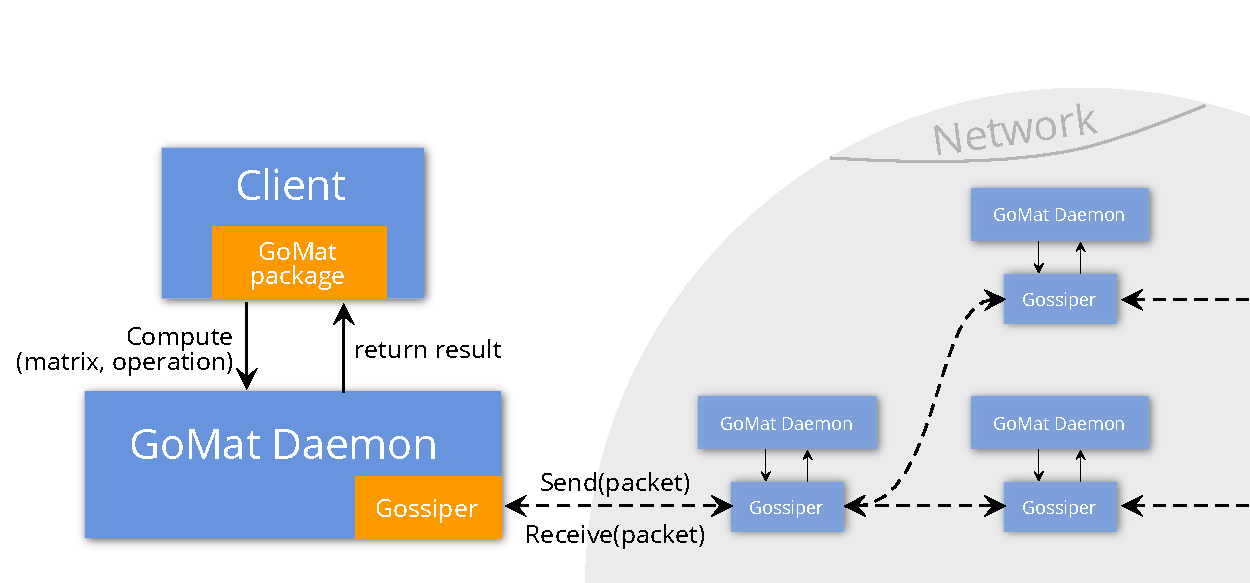
\includegraphics[width=.95\textwidth]{global_view.pdf}
        \caption{Global view}
        \label{glbView}
    \end{figure}
    \begin{figure}[!ht]
        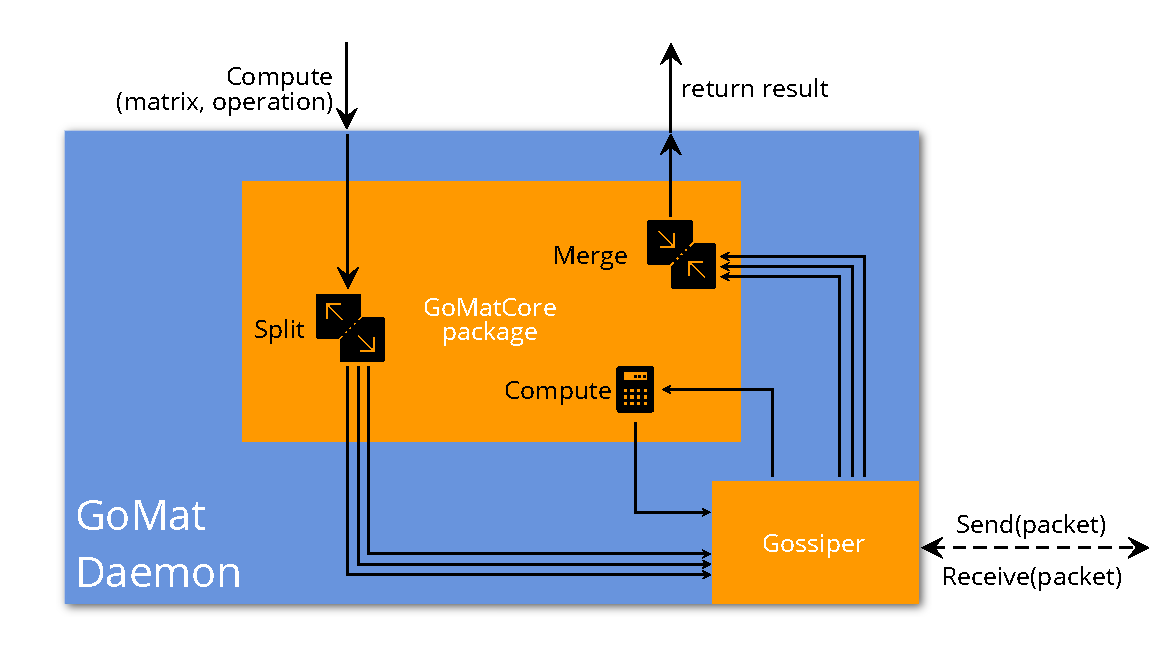
\includegraphics[width=.95\textwidth]{daemon_view.pdf}
        \caption{Daemon architecture}
        \label{daemonView}
    \end{figure}
    
    \section{Daemon}
    When a user wants to join a \Gomat network, it has to run the dedicated daemon. The daemon is the main component of the application. It splits and merges matrices, executes computations and communicates with other peers. For this last point, it uses a \Gossiper network.

    A \Gomat peer is not a \Gossiper peer, but contains a \Gossiper peer that it uses to send and receive messages. Our \Gomat application uses the \Gossiper as a transport layer (layer 4).

    \subsection{GUI}
    Once the daemon is running, it is not automatically connected to a \Gomat network. The user has to open a web browser and go on \url{http://localhost:8080} (can be modified in a configuration file) to add some peers to be connected on a
    \Gomat network.
    
    On the \texttt{GUI}, the client can change the maximum number of computations his computer can do at a time. He can see
    the number of computation his computer have done, check the peers he knows, see our ratio
    ($r =$ number of computation tasks sent/{number of computation tasks computed}).

    \section{API}
    Our API is a \Go package which is used to communicate with the daemon. When a user wants to compute an operation between to big matrices, he calls:\\
    \texttt{Gomat.compute(matrix1, matrix2 Matrix, operation Gomat.Operation)(result Matrix, err error)}\\
    This function is blocking.

    If there is no \Gomat daemon running on the computer, \texttt{Gomat.compute} returns an error.

    \subsection{Communications between API and Daemon}
    The application using the API and the Daemon are running on the same computer. Thus, there is no need to use the network (i.e. the loopback interface).
    We use \texttt{Inter-Process Communication (IPC) sockets} to send information between the daemon and the API.

    \section{Failure detection and management}
    Since it is a decentralised system where one peer delegates part of its job to others, it is essential to detect failures, manage them, and implement methods that make the system more resilient.

    It must be noted that failure detection and management work both ways. For a given computation, the gossiper that wants its job done must detect failing peers, so that it does not have to wait forever for their reply, but ‘computing’ gossiper want to detect if the node that send them tasks fails, so that they can drop the job and reallocate their resources.

    \subsection{Detecting failures}
    To manage failures, we first need to detect them.

    When \texttt{Gomat.compute} is used, the \Gomat daemon will first check that all of its peers are working. To that effect, it will send them a particular message and will wait for an acknowledgement. If after some time, some do not reply, they will be considered to have failed, will be removed from the list of peers, and no task will be sent to them.

~~

    Whenever a ‘master’ gossiper splits a computation and sends it to peers for computing, it creates a routine for each contacted gossiper, that listens and writes to it.
When a gossiper receives the job, it acknowledges it by sending an answer to the master gossiper.
Then, the master will send back a message to the gossiper, who will reply, and so one.

    If at any point, a gossiper times out when listening (i.e. it does not receive an answer fast enough), the other node is considered to have failed.

~~

    It must be noted that such a message coming from an unknown peer is received, it will be added to the list of potential peers.

    \subsection{Failure management}
    When a gossiper $g$ finds that another one, $a$, has failed, it will be removed from the list of peers, the routine created to communicate with $a$ will be killed and one of the three will occur:

\begin{itemize}
\item If $a$ was doing some computation for $g$, $g$ will split the computation between its remaining peers.
\item If $g$ was doing some computation for $a$, $a$ will stop its computation.
\item In any other case, nothing more will be done. 
\end{itemize}

    \subsection{Making the system more resilient}
    If a gossiper $g$ receives a task and has enough idle peers, it can redistribute some of it amongst them. There must be some wait time (maybe they have all received subtasks from the same job, but because of delays, $g$ still sees them as idle).
In that case, the ‘master’ peer must be informed of their computations, they will be added to its peers, and as for others, it must now detect their failures.

    Then, if $g$ crashes, not all of the computations sent to him will have to be redone, since some subtasks are now processed by its peers.

    The master node will also be able to add gossipers to its list of known peers, and the network will be more robust.

\section{Conclusion}
    These specifications are meant to change, since it is only a first draft.
    

\end{document}